\documentclass[tikz,border=10pt]{standalone}
\usepackage{tikz}
\usetikzlibrary{trees,decorations.pathreplacing}

\begin{document}

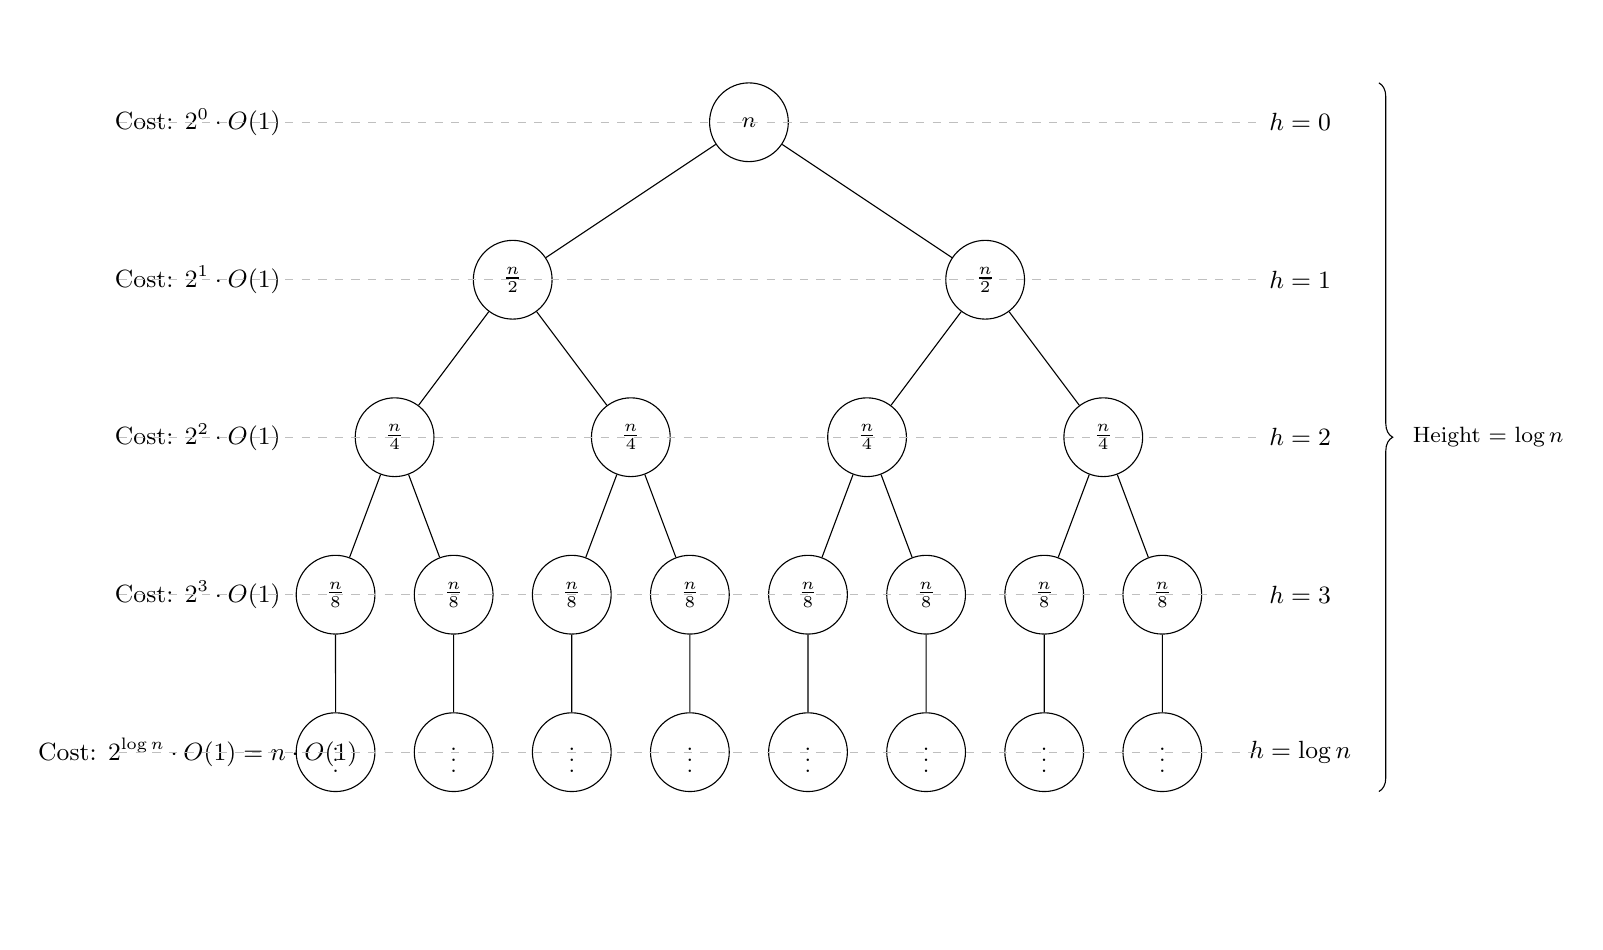
\begin{tikzpicture}[
    level distance=20mm,
    every node/.style={circle,draw,minimum size=10mm,font=\footnotesize},
    level 1/.style={sibling distance=60mm},
    level 2/.style={sibling distance=30mm},
    level 3/.style={sibling distance=15mm},
    level 4/.style={sibling distance=8mm}
]

% Main tree
\node {$n$}
  child {node {$\frac{n}{2}$}
    child {node {$\frac{n}{4}$}
        child {node {$\frac{n}{8}$}
            child {node {$\vdots$}}
        }
        child {node {$\frac{n}{8}$}
            child {node {$\vdots$}}
        }
    }
    child {node {$\frac{n}{4}$}
        child {node {$\frac{n}{8}$}
            child {node {$\vdots$}}
        }
        child {node {$\frac{n}{8}$}
            child {node {$\vdots$}}
        }
    }
  }
  child {node {$\frac{n}{2}$}
    child {node {$\frac{n}{4}$}
        child {node {$\frac{n}{8}$}
            child {node {$\vdots$}}
        }
        child {node {$\frac{n}{8}$}
            child {node {$\vdots$}}
        }
    }
    child {node {$\frac{n}{4}$}
        child {node {$\frac{n}{8}$}
            child {node {$\vdots$}}
        }
        child {node {$\frac{n}{8}$}
            child {node {$\vdots$}}
        }
    }
  };

% Height labels (right side)
\node[draw=none, font=\small] at (7, 0) {$h = 0$};
\node[draw=none, font=\small] at (7, -2) {$h = 1$};
\node[draw=none, font=\small] at (7, -4) {$h = 2$};
\node[draw=none, font=\small] at (7, -6) {$h = 3$};
\node[draw=none, font=\small] at (7, -8) {$h = \log n$};

% Cost labels (left side)
\node[draw=none, font=\small] at (-7, 0) {Cost: $2^0 \cdot O(1)$};
\node[draw=none, font=\small] at (-7, -2) {Cost: $2^1 \cdot O(1)$};
\node[draw=none, font=\small] at (-7, -4) {Cost: $2^2 \cdot O(1)$};
\node[draw=none, font=\small] at (-7, -6) {Cost: $2^3 \cdot O(1)$};
\node[draw=none, font=\small] at (-7, -8) {Cost: $2^{\log n} \cdot O(1) = n \cdot O(1)$};

% Total height bracket
\draw[decorate, decoration={brace, amplitude=5pt}] 
    (8, 0.5) -- (8, -8.5) node[midway, right=8pt, draw=none] {Height = $\log n$};

% Horizontal dashed lines to show levels
\draw[dashed, gray!50] (-8, 0) -- (6.5, 0);
\draw[dashed, gray!50] (-8, -2) -- (6.5, -2);
\draw[dashed, gray!50] (-8, -4) -- (6.5, -4);
\draw[dashed, gray!50] (-8, -6) -- (6.5, -6);
\draw[dashed, gray!50] (-8, -8) -- (6.5, -8);

\end{tikzpicture}

\end{document}